\newpage
\section{Evaluation of Text Retrieval Systems}

%----------------------------------------
\subsection{The Cranfield Evaluation Methodology}

A methodology for laboratory testing of system components developed in 1960s. General idea is to build reusable test collections and define measures. A test collection can then be reused many times to compare different systems.
\begin{itemize}
\item A sample collection of documents (simulate real document collection)
\item A sample set of queries/topics (simulate user queries)
\item Relevance judgments (ideally made by users who formulated the queries) => ideal ranked list
\item  Measures to quantify how well a system’s result matches the ideal ranked list
\end{itemize}


%----------------------------------------
\subsection{Basic Measures}
\subsubsection{Evaluating a Set of Retrieved Docs}

\begin{center}
  \begin{tabular}{ | l | c | c | }
    \hline
    & \textbf{Retrieved} & \textbf{Not Retrieved} \\    
    \hline    
    \textbf{Relevant}     & a & b \\
    \textbf{Not Relevant} & c & d \\
    \hline  
  \end{tabular}
\end{center}

\begin{itemize}
\item Precision: are the retrieved results all relevant?
\begin{equation*}
Precision = \frac{a}{a+c}
\end{equation*}
\item Recall: have all the relevant documents been retrieved?
\begin{equation*}
Recall = \frac{a}{a+b}
\end{equation*}
\item In reality, high recall tends to be associated with low precision
\end{itemize}


%----------------------------------------
\subsubsection{Combine Precision and Recall: F-Measure}

\begin{equation*}
F_\beta = \frac{1}{\dfrac{\beta^2}{\beta^2+1}\dfrac{1}{R} + \dfrac{1}{\beta^2+1}\dfrac{1}{P}} = \frac{(\beta^2+1)\cdot P \cdot R}{\beta^2 \cdot P + R}
\end{equation*}

\begin{itemize}
\item $P$ - precision
\item $R$ - recall
\item $\beta$ - parameter, often set to 1:
\end{itemize}

\begin{equation*}
F_1 = \dfrac{2 \cdot P \cdot R}{P+R}
\end{equation*}


%----------------------------------------
\newpage
\subsection{Evaluating a Ranked List}
\subsubsection{Evaluating Ranking: Precision-Recall (PR) Curve}
\begin{itemize}
\item Total number of relevant documents in collection: $a+b = 10$
\item Number of retrieved documents: $a+c = 10$
\end{itemize}

\begin{multicols}{2}
\begin{center}
  \texttt{  
  \begin{tabular}{ | c | c | c | }
    \hline
    \textbf{Relevance} & \textbf{Precision} & \textbf{Recall} \\    
    \hline    
    \textbf{D1 +} & 1/1 & 1/10 \\ 
    \textbf{D2 +} & 2/2 & 2/10 \\
    \textbf{D3 -} & 2/3 & 2/10 \\
    \textbf{D4 -} & 2/4 & 2/10 \\
    \textbf{D5 +} & 3/5 & 3/10 \\
    \textbf{D6 -} & 3/6 & 3/10 \\
    \textbf{D7 -} & 3/7 & 3/10 \\
    \textbf{D8 +} & 4/8 & 4/10 \\
    \textbf{D9 -} & 4/9 & 4/10 \\
    \textbf{D10 -} & 4/10 & 4/10 \\
    \hline  
  \end{tabular}
  }
\end{center}

\columnbreak

\begin{figure}[H]
    \centering
    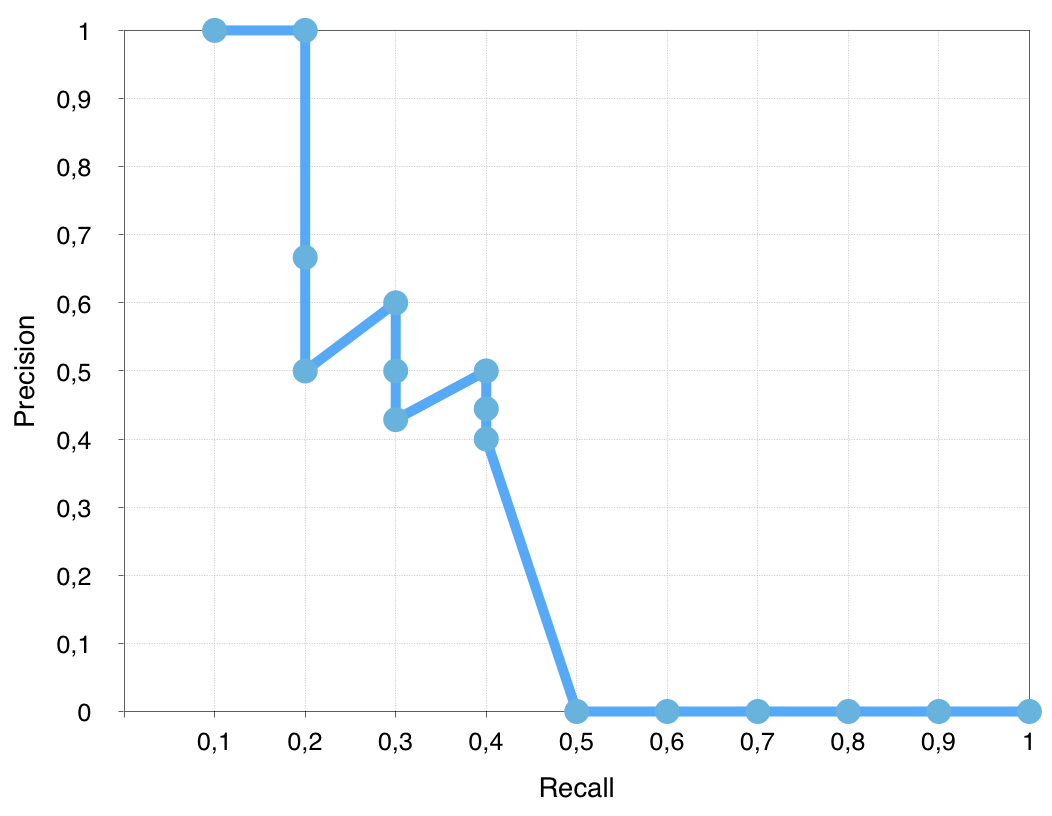
\includegraphics[width=\linewidth]{PR.png}
\end{figure}
\end{multicols}


%----------------------------------------
\subsubsection{How to Summarize a Ranking}
\href{http://en.wikipedia.org/wiki/Information_retrieval#Average_precision}{Average Precision} is sensitive to the rank of each relevant document:
\begin{equation*}
AveP = \dfrac{\sum\limits_{k=1}^{a+c} P(k) \cdot rel(k)}{a+b} = \sum\limits_{k=1}^{a+c} P(k) \cdot \Delta r(k)
\end{equation*}
\begin{itemize}
\item $a+c$ - number of retrieved documents
\item $a+b$ - total number of relevant documents in collection
\item $P(k)$ - the precision at cut-off $k$ in the list
\item $rel(k)$ - indicator function equaling 1 if the item at rank $k$ is a relevant document, zero otherwise
\item $\Delta r(k)$ - the change in recall that happened between cut-off $k-1$ and cut-off $k$
\end{itemize}

In special case, when there’s only one relevant document in the collection (e.g., known item search): 
\begin{itemize}
\item Average Precision = \textbf{Reciprocal Rank} = 1/r, where r is the rank position of the single relevant doc
\end{itemize}

%----------------------------------------
\subsubsection{Mean Average Precision (MAP)}
In case of multiple queries:
\begin{itemize}
\item MAP = arithmetic mean of average precision over a set of queries 
\begin{equation*}
MAP = \frac{\sum\limits_{q=1}^{N}AveP(q)}{N}\text{,\; where $N$ is the number of queries}
\end{equation*}

\item \href{http://trec.nist.gov/pubs/trec15/appendices/CE.MEASURES06.pdf}{gMAP} = geometric mean of average precision over a set of queries
\begin{equation*}
gMAP = \sqrt[N]{\prod_{q=1}^{N}AveP(q)} = \exp \frac{\sum\limits_{q=1}^{N} \log \big(AveP(q)\big)}{N}
\end{equation*}
\end{itemize}

%----------------------------------------
\subsubsection{Summary}
\begin{itemize}
\item Precision-Recall curve characterizes the overall accuracy of a ranked list
\item The \textbf{actual} utility of a ranked list depends on how many top-ranked results a user would examine
\item Average Precision is the standard measure for comparing two ranking methods
\begin{itemize}
\item Combines precision and recall
\item Sensitive to the rank of \textbf{every} relevant document
\end{itemize}
\end{itemize}

%----------------------------------------
\subsection{Multi-level Relevance Judgments}
\href{http://en.wikipedia.org/wiki/Discounted_cumulative_gain}{Discounted cumulative gain (DCG)} is a measure of ranking quality. Two assumptions are made in using DCG and its related measures:
\begin{itemize}
\item Highly relevant documents are more useful when appearing earlier in a search engine result list (have higher ranks)
\item Highly relevant documents are more useful than marginally relevant documents, which are in turn more useful than irrelevant documents.
\end{itemize}

For a rank position p:
\begin{itemize}
\item \textbf{Cumulative Gain}: $\mathrm{CG_p} = \sum\limits_{i=1}^{p}rel_i$, where $rel_i$ is the graded relevance of the result at position $i$
\item \textbf{Discounted Cumulative Gain}: $\mathrm{DCG_p} = rel_1 + \sum\limits_{i=2}^{p}\dfrac{rel_i}{\log_{2}i}$
\item Alternative version of \textbf{Discounted Cumulative Gain}: $\mathrm{DCG_p} = \sum\limits_{i=1}^{p}\dfrac{2^{rel_i}-1}{\log_{2}(i+1)}$
\item \textbf{Normalized DCG}: $\mathrm{nDCG_p} = \dfrac{\mathrm{DCG_p}}{\mathrm{IDCG_p}}$, where $\mathrm{IDCG_p}$ is an Ideal DCG (the maximum possible DCG till position $p$)
\end{itemize}

For example, each document is to be judged on a scale of 0-3 with 0 meaning irrelevant, 3 meaning completely relevant, and 1 and 2 meaning <<somewhere in between>>

\begin{center}
  \texttt{  
  \begin{tabular}{ | c | c | c | }
    \hline
    Document & $rel_i$ & $\dfrac{rel_i}{\log_{2}i}$ \\    
    \hline    
    \textbf{D1} & 3 & - \\ 
    \textbf{D2} & 2 & 2 \\
    \textbf{D3} & 3 & 1.892 \\
    \textbf{D4} & 0 & 0 \\
    \textbf{D5} & 1 & 0.431 \\
    \textbf{D6} & 2 & 0.774 \\
    \hline  
  \end{tabular}
  }
\end{center}

\begin{itemize}
\item $\mathrm{DCG_6} = rel_{1} + \sum_{i=2}^{6} \frac{rel_{i}}{\log_{2}i} = 3 + (2 + 1.892 + 0 + 0.431 + 0.774) = 8.10$
\item $\mathrm{IDCG_{6}} = 8.69\quad (rel_i = {3,3,2,2,1,0})$
\item $\mathrm{nDCG_{6}} = \frac{DCG_{6}}{IDCG_{6}} = \frac{8.10}{8.69} = 0.932$
\end{itemize}

%----------------------------------------
\subsection{Statistical Significance Tests}
\begin{figure}[H]
    \centering
    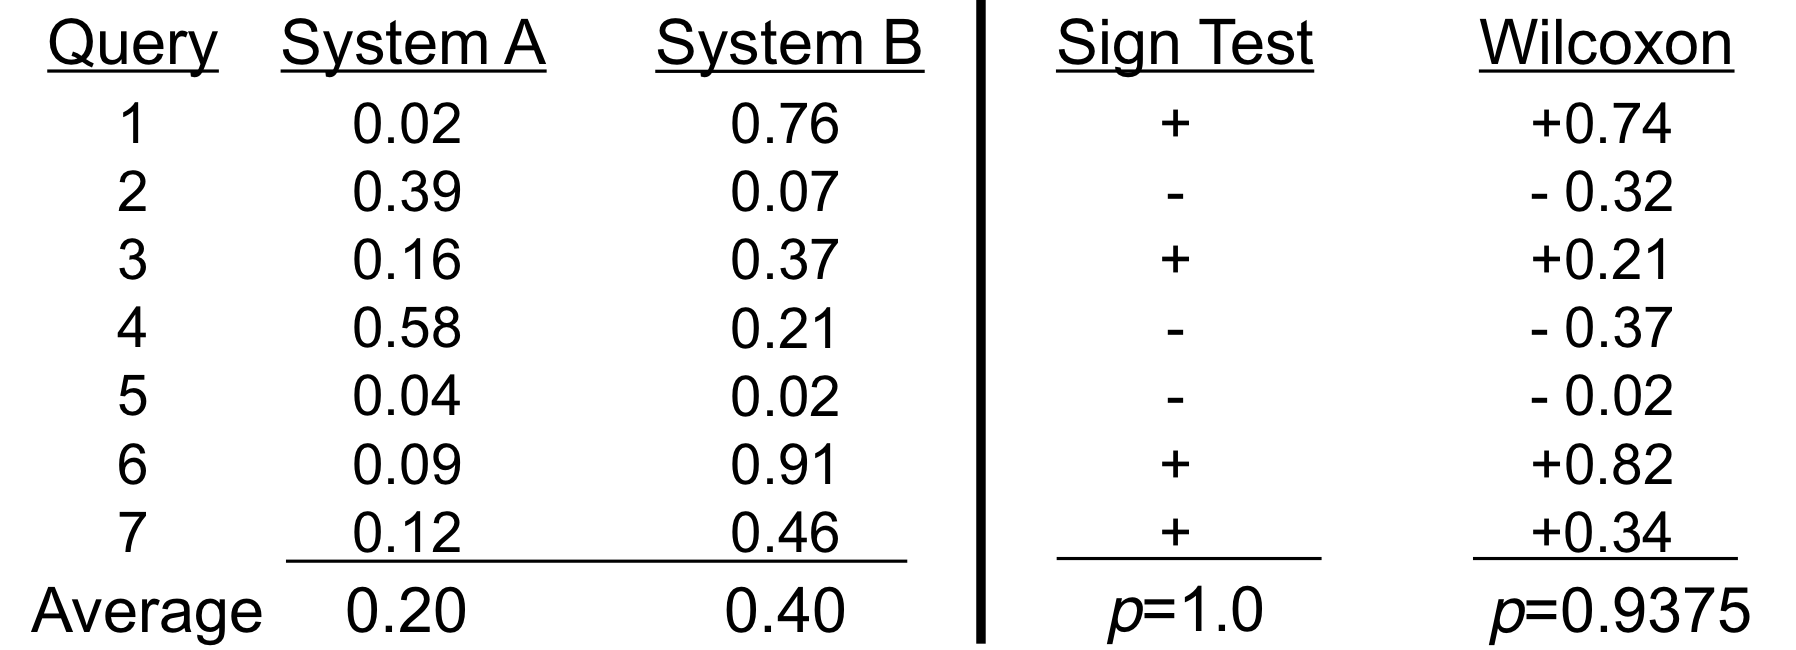
\includegraphics[width=0.9\linewidth]{statistical_significance_test.png}
\end{figure}

\textrussian{
\textbf{Нулевая гипотеза} - гипотеза об отсутствии взаимосвязи или корреляции между исследуемыми переменными, об отсутствии различий (однородности) в распределениях (параметрах распределений) двух и/или более выборках.
\begin{itemize}
\item H0: median difference between the pairs is zero
\item H1: median difference is not zero.
\end{itemize}


\subsubsection{Sign test}
\href{https://ru.wikipedia.org/wiki/Критерий_знаков}{Критерий знаков} используется при проверке нулевой гипотезы о равенстве медиан двух непрерывно распределенных случайных величин

Рассмотрим две непрерывно распределенные случайные величины $X$ и $Y$, и пусть нулевая гипотеза выполняется, то есть их медианы равны. Тогда $p=\mathbb P(X>Y)=0.5$. Иными словами, каждая из случайных величин равновероятно больше другой. 

Рассмотрим пару связных выборок $\{(x_1,y_1),\ldots,(x_n,y_n)\}$. Будем считать, что в выборке нет элементов, для которых $x_i=y_i$ (иначе уберем эти элементы из выборки). Построим статистику $w$, равную числу элементов в выборке, при которых $x_i>y_i$. При выполнении нулевой гипотезы, эта величина имеет биномиальное распределение: $w\sim B(n,0.5)$ с функцией вероятности 
\begin{equation*}
p_Y(k) \equiv \mathbb{P}(Y = k) = \binom{n}{k}\, p^k q^{n-k}, \ \ k=0,\ldots, n, 
\end{equation*}
где $\dbinom{n}{k} = C_n^i = \dfrac{n!}{(n-k)! \, k!}$ — биномиальный коэффициент.

Для применения критерия необходимо вычислить <<левый хвост>> биномиального распределения до $w$: 
\begin{equation*}
b=2^{-n}\sum_{i=0}^w \binom{n}{i}
\end{equation*}
Согласно критерию, при уровне значимости $\alpha$: если $b \notin \left[ \alpha/2,\, 1-\alpha/2 \right]$, то нулевая гипотеза $p \ne 0.5$ отвергается.
}


\subsubsection{Wilcoxon signed-rank test}

\href{http://en.wikipedia.org/wiki/Wilcoxon_signed-rank_test}{The Wilcoxon signed-rank test} is a non-parametric statistical hypothesis test used when comparing two related samples or repeated measurements on a single sample to assess whether their population mean ranks differ.

Let $N$ be the sample size, the number of pairs. Thus, there are a total of $2N$ data points. For $i = 1, \dots , N$, let $x_{1,i}$ and $x_{2,i}$ denote the measurements.
\begin{itemize}
\item For $i = 1, \dots , N$, calculate $|x_{2,i} - x_{1,i}|$ and $\sign(x_{2,i} - x_{1,i})$.
\item Exclude pairs with $|x_{2,i} - x_{1,i}| = 0$. Let $N_r$ be the reduced sample size.
\item Order the remaining $N_r$ pairs from smallest absolute difference to largest absolute difference, $|x_{2,i} - x_{1,i}|$.
\item Rank the pairs, starting with the smallest as 1. Ties receive a rank equal to the average of the ranks they span. Let $R_i$ denote the rank.
\item Calculate the test statistic $W$, the absolute value of the sum of the signed ranks:
\begin{equation*}
W = \left|\sum_{i=1}^{N_r} [\sign(x_{2,i} - x_{1,i}) \cdot R_i]\right|
\end{equation*}
\item As $N_r$ increases, the sampling distribution of $W$ converges to a normal distribution. Thus,
\begin{itemize}
\item For $N_r \geqslant 10$, a z-score can be calculated as $z = \frac{W - 0.5}{\sigma_W}, \sigma_W = \sqrt{\frac{N_r(N_r + 1)(2N_r + 1)}{6}}$. If $z > z_{critical}$ then reject $H_0$
\item For $N_r < 10$, $W$ is compared to a critical value from a reference table. If $W \geqslant W_{critical, N_r}$ then reject $H_0$
\end{itemize}
\end{itemize}

Example:
\begin{figure}[H]
    \centering
    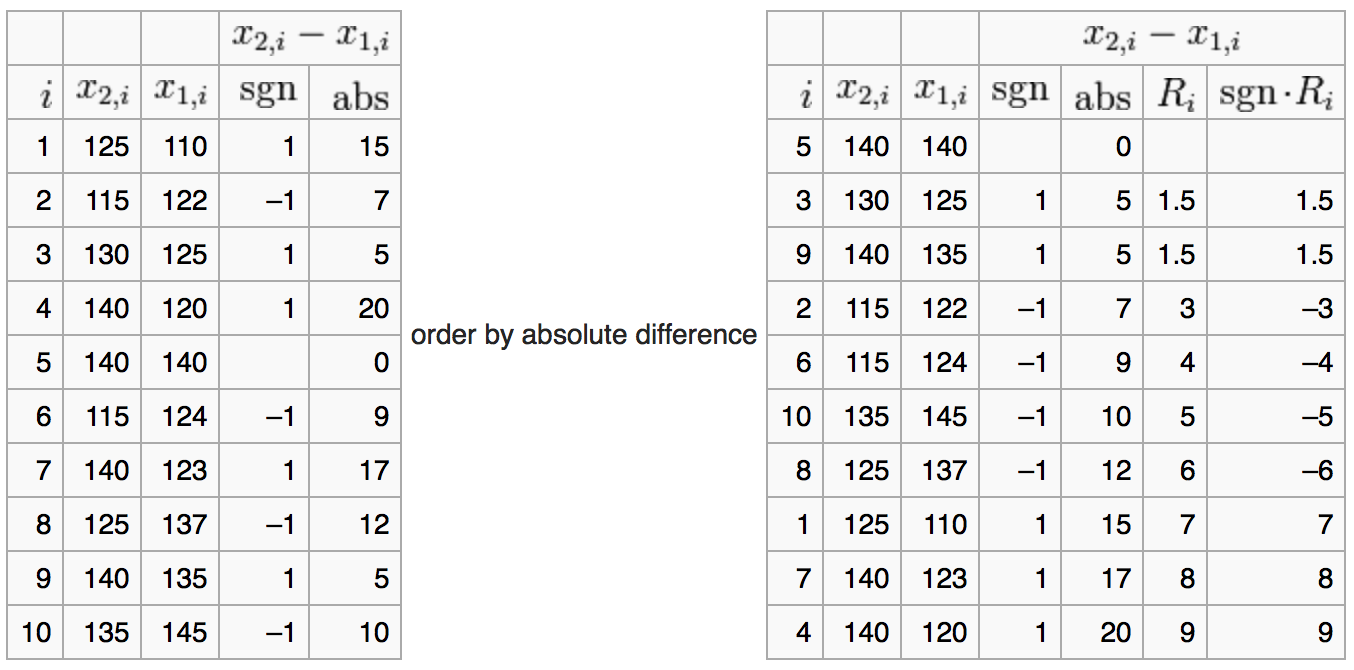
\includegraphics[width=0.9\linewidth]{wilcoxon.png}
\end{figure}

Notice that pairs 3 and 9 are tied in absolute value. They would be ranked 1 and 2, so each gets the average of those ranks, 1.5.\\

$N_r = 10 - 1 = 9, W = |1.5+1.5-3-4-5-6+7+8+9| = 9$

$W < W_{\alpha = 0.05, 9} = 39 \; \therefore \; \text{fail to reject } H_0$

%----------------------------------------
\subsection{Pooling: Avoid Judging all Documents}
Pooling strategy:
\begin{itemize}
\item Choose a diverse set of ranking methods (TR systems)
\item Have each to return top-K documents
\item Combine all the top-K sets to form a pool for human assessors to judge
\item Other (unjudged) documents are usually assumed to be non-relevant (though they don’t have to)
\end{itemize}

Pooling strategy is okay for comparing systems that contributed to the pool, but problematic for evaluating new systems.

%----------------------------------------
\subsection{Summary of TR Evaluation}
Evaluation is extremely important:
\begin{itemize}
\item TR is an empirically defined problem
\item Inappropriate experiment design misguides research and applications 
\item Make sure to get it right for your research or application
\end{itemize}

Cranfield evaluation methodology is the main paradigm:
\begin{itemize}
\item MAP and nDCG: appropriate for comparing ranking algorithms
\item Precision@10docs is easier to interpret from a user’s perspective
\end{itemize}

Not covered:
\begin{itemize}
\item A-B Test [Sanderson 10] 
\item User studies [Kelly 09]
\end{itemize}

%----------------------------------------
\subsection{Recommended reading}
\begin{itemize}
\item Donna Harman, <<Information Retrieval Evaluation. Synthesis Lectures on Information Concepts, Retrieval, and Services>>, Morgan \& Claypool Publishers 2011
\item Mark Sanderson, <<Test Collection Based Evaluation of Information Retrieval Systems>>. Foundations and Trends in Information Retrieval 4(4): 247-375 (2010)
\item  Diane Kelly, <<Methods for Evaluating Interactive Information Retrieval Systems with Users>>. Foundations and Trends in Information Retrieval 3(1-2): 1-224 (2009)
\end{itemize}




